%! Author = timbe
%! Date = 05.02.2024

% Preamble
\documentclass[12pt]{article}

% Packages
\usepackage[left=3.0cm, right=1.5cm, top=2.0cm, bottom=2.0cm]{geometry}

\usepackage[utf8]{inputenc}
\usepackage[T2A]{fontenc}
\usepackage[russian]{babel}
\usepackage{amsmath, amsfonts, amssymb}
\usepackage{graphicx}
\usepackage{wrapfig}
\usepackage{fancyhdr}
\usepackage[shortlabels]{enumitem}
\usepackage{svg}
\usepackage{amstex}
\usepackage{colortbl}
\usepackage{hyperref}
\usepackage{calc}
\usepackage{pifont}

\renewcommand{\vec}{\textbf}
\newcommand{\cross}{\times}

\pagestyle{fancy}
\fancyhead[L]{Работа №4.7.1}
\fancyhead[R]{Белинский Т.Д.\quad Б05-206}

% Document
\begin{document}
    \section*{4.7.1. ДВОЙНОЕ ЛУЧЕПРЕЛОМЛЕНИЕ}
    \ \par
    \textbf{Цель работы:} изучение зависимости показателя преломления
    необыкновенной волны от направления в двоякопреломляющем кристалле;
    определение главных показателей преломления в кристалле.\par
    \textbf{Оборудование:} гелий-неоновый лазер, вращающийся столик с неподвижным лимбом,
    призма из исландского шпата, поляроид.

    \subsection*{Теоретическая часть}
    \ \par
    В некоторых кристаллах потенциальные ямы, в которых находятся электроны вблизи узлов решетки,
    не являются симметричными.
    Причем всегда можно выбрать систему координат, чтобы потенциальная энергия электрона при
    малых отклонениях имела следующий вид
    \[U = a_x x^2 a_y y^2 a_z z^2.\]
    Если два коэффициента равны $a_y = a_z = a_{\perp},\  a_x = a_{\paral}$, то кристалл называют
    одноосным, а ось $x$ -- главной оптической осью.

    По сколько величины отклонений электрона от положения равновесия вдоль разных осей зависят
    от соответствующих коэффициентов $a_x, a_y, a_z$, то в случае одноосного кристалла вектор поляризации $\vec{P}$
    будет неколлиниарен вектору напряженности внешнего электрического поля $\vec{E}$:
    \begin{equation}
        \label{eq:eq1}
        \vec{P} = \alpha_{\paral} \vec{E}_{\parallel} + \alpha_{\perp} \vec{E}_{\perp},\quad
        \vec{D} = \varepsilon_{\parallel} \vec{E}_{\parallel} + \varepsilon_{\perp} \vec{E}_{\perp}.
    \end{equation}

    Записав волны в общем виде
    \begin{equation*}
        \vec{E} = \vec{E}_0 \,e^{i(wt - \vec{k}\vec{r})},\quad \vec{H} = \vec{H}_0\,e^{i(wt - \vec{k}\vec{r})},\quad
        \vec{D} = \vec{D}_0\,e^{i(wt - \vec{k}\vec{r})}
    \end{equation*}
    и подставив в уравнения Максвелла
    \begin{equation*}
        rot\, \vec{H} = \frac{1}{c} \frac{\partial \vec{D}}{\partial t},\quad
        rot\, \vec{E} = -\frac{1}{c} \frac{\partial \vec{H}}{\partial t},
    \end{equation*}
    получим
    \begin{equation}
        \label{eq:eq2}
        \vec{D} = -\frac{c}{w} \vec{k} \cross \vec{H},\quad \vec{H} = \frac{c}{w} \vec{k} \cross \vec{E}.
    \end{equation}

    \begin{wrapfigure}[9]{r}{0.5\linewidth}
        \label{fig:fig1}
        \centering
        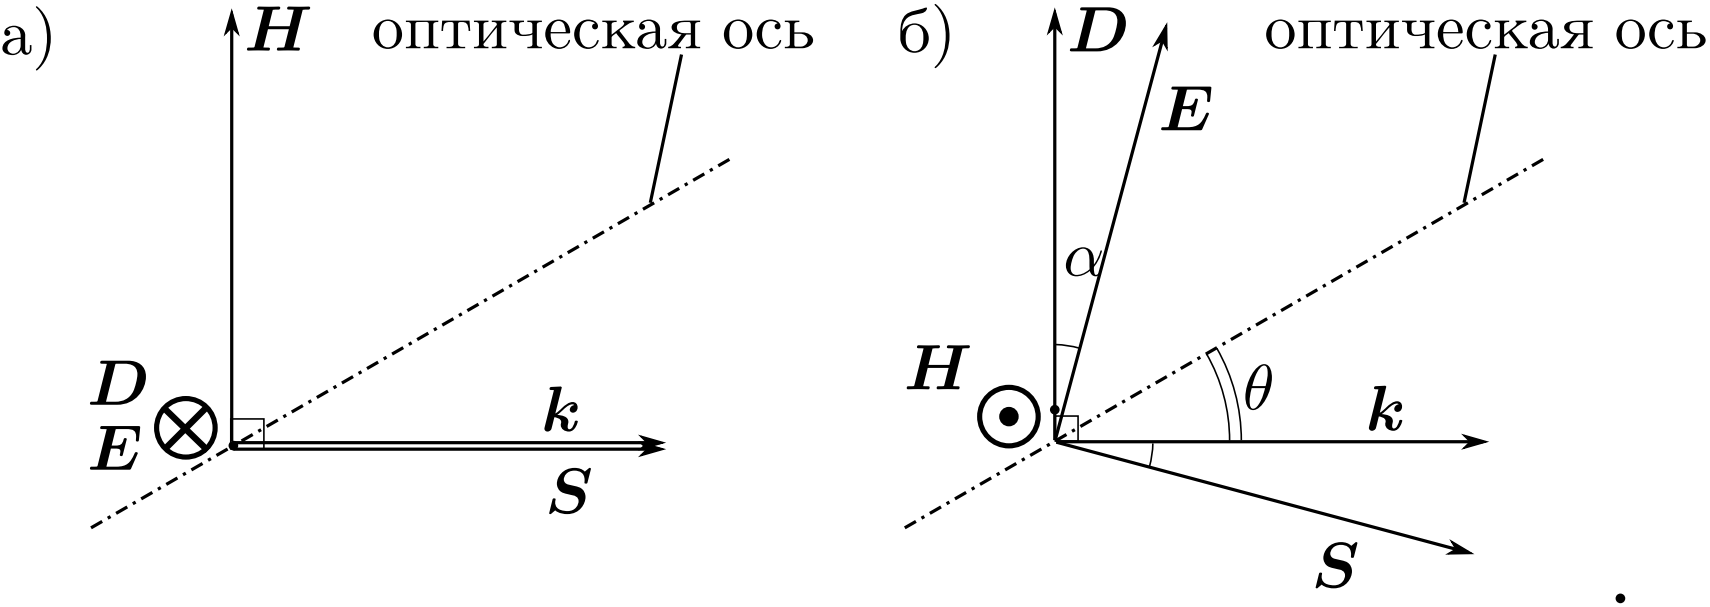
\includegraphics[width=\linewidth]{pic/vecdiag}
        \caption{Обыкновенная (a) и необыкновенная (b) волны}
    \end{wrapfigure}
    Главной плоскостью будем называть плоскость, образованную оптической осью и волновым вектором $\vec{k}$.
    Анализ уравнений\ \eqref{eq:eq2} показывает, что возможны два расположения векторов
    $\vec{D}, \vec{E}, \vec{k}, \vec{H}$ друг относительно друга:
    \begin{enumerate}[(a)]
        \item $\vec{D} = \varepsilon_{\perp} \vec{E}_{\perp}$ -- $\vec{D}$ перпендикулярен главной плоскости
        \item $\vec{D} = \varepsilon_{\parallel} \vec{E}_{\parallel} + \varepsilon_{\perp} \vec{E}_{\perp}$ --
        $\vec{D}$ лежит в главной плоскости
    \end{enumerate}

    В первом случае волна называется обыкновенной, а во втором -- необыкновенной.
    Поскольку уравнения Максвелла линейны, то в общем случае любое монохроматическое поле в кристалле
    можно представить как суперпозицию обыкновенной и необыкновенной волн.

    Выразим фазовую скорость $v = \frac{w}{k}$ для волны в анизотропной среде
    \begin{equation*}
        \eqref{eq:eq2} \Rightarrow v = \frac{cH}{D} = \frac{cE\cos{\alpha}}{H} \Rightarrow
    \end{equation*}
    \begin{equation}
        \label{eq:eq3}
        \Rightarrow v = \sqrt{\frac{c^{2E}\cos{\alpha}}{D}} = c\sqrt{\frac{\vec{E}\cdot\vec{D}}{D^2}}.
    \end{equation}

    Тогда в соответствии с формулой\ \eqref{eq:eq3} фазовая скорость обыкновенной волны
    \begin{equation}
        \label{eq:eq4}
        v_o = \frac{c}{\sqrt{\varepsilon_{\perp}}} = \frac{c}{n_o}.
    \end{equation}

    Для необыкновенной волны
    \begin{equation*}
        \vec{E}\cdot\vec{D} = \varepsilon_{\parallel} E_{\parallel}^2 + \varepsilon_{\perp} E_{\perp}^2 =
        \frac{D_{\parallel}^2}{\varepsilon_{\parallel}} +  \frac{D_{\perp}^2}{\varepsilon_{\perp}} \Rightarrow
    \end{equation*}
    \begin{equation}
        \label{eq:eq5}
        \Rightarrow
        v_e = c\sqrt{\frac{\sin^2{\theta}}{\varepsilon_{\parallel}} + \frac{\cos^2{\theta}}{\varepsilon_{\perp}}} =
        \frac{c}{n(\theta)}.
    \end{equation}

    Величины $n_o = \sqrt{\varepsilon_{\perp}},\ n_e = \sqrt{\varepsilon_{\parallel}}$
    называют главными показателями преломления.
    Используя эти обозначения можно записать формулу для $n(\theta)$ из уравнения\ \eqref{eq:eq5}
    \begin{equation}
        \label{eq:eq6}
        n^2(\theta) = \left(\frac{\sin^2{\theta}}{n_e^2} +
        \frac{\cos^2{\theta}}{n_o^2}\right)^{-1}.
    \end{equation}
    При условии $n_o - n_e \l n_o, n_e$ формулу\ \eqref{eq:eq6} можно упростить
    \begin{equation}
        \label{eq:eq7}
        n(\theta) \approx n_o + (n_o - n_e)\cos^2{\theta}
    \end{equation}

    \subsection*{Экспериментальная установка}
    \ \par
    \begin{wrapfigure}[12]{r}{0.55\linewidth}
        \label{fig:fig2}
        \centering
        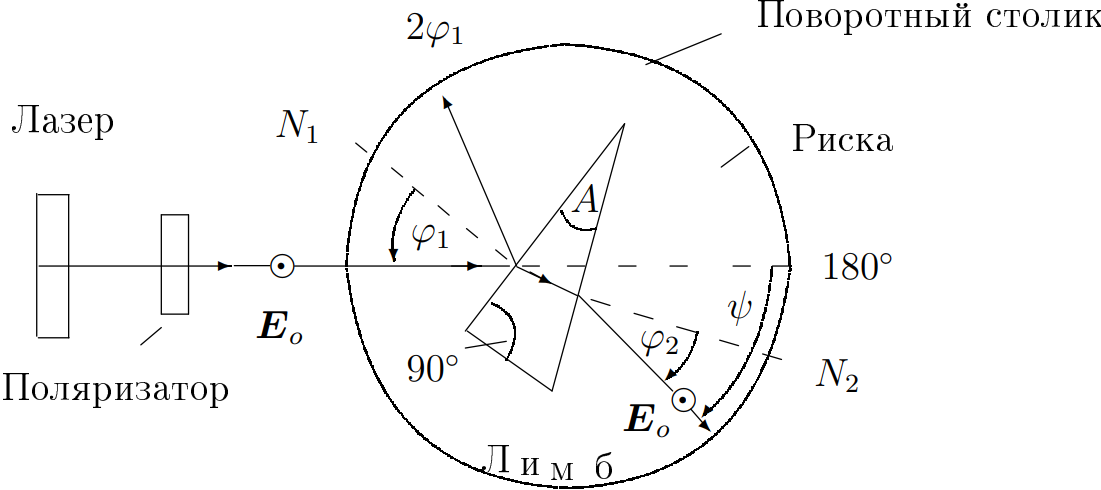
\includegraphics[width=\linewidth]{pic/setup}
        \caption{Ход лучей в призме}
    \end{wrapfigure}
    Исследуемая призма, изготовленная из исландского шпата, закреплена в центре поворотного столика.
    Оптическая ось кристалла параллельна длинному катету и верхней поверхности призмы.
    Преломляющий угол $A$ можно рассчитать, если известны угловые координаты лучей отраженных от
    преломляющих граней.

    Из рис.2 можно получить
    \begin{equation}
        \varphi_2 = A + \psi - \varphi_1,
        \label{eq:eq8}
    \end{equation}
    где $\psi$ -- угол между первоначальным направлением и направлением преломленного луча --
    определяется по разности отсчетов на лимбе между точкой, куда попадает луч в отсутствии призмы,
    и точкой, куда попадает преломленный луч.

    При монотонном увеличении угла падения $\varphi_1$, угол $\psi$ сначала монотонно уменьшается,
    а затем монотонно увеличивается.
    Наименьшее значение угла $\psi_m$ достигается при $\varphi_1 = \varphi_2$.
    Тогда показатель преломления $n$ можно рассчитать по формуле
    \begin{equation}
        \label{eq:eq9}
        n = \frac{\sin{\left(\frac{\psi_m + A}{2}\right)}}{\sin{\frac{A}{2}}}.
    \end{equation}

    Строго говоря, формулой\ \eqref{eq:eq9} в случае анизотропной призмы можно воспользоваться
    только для обыкновенной волны.
    Но если учесть, что угол при вершине призмы мал и при угле наименьшего отклонения преломленный луч
    в призме распространяется под углом к оси кристалла, близким к $\pi/2$, то формулу\ \eqref{eq:eq9}
    можно использовать в качестве оценки $n_e$.

    \subsection*{Результаты и обработка}
    \begin{enumerate}
        \item Измерение преломляющего угла призмы $A$:
        \begin{enumerate}
            \item устанавливаем луч, отраженный от длинного катета, на отметку $10^{\circ}$ по лимбу;
            \item записываем соответствующий отсчет по риске;
            \item повторяем пункты (a), (b),
            изменяя координату отраженного луча от $10^{\circ}$ до $140^{\circ}$ с шагом $10^{\circ}$;
            \item повторяем пункты (a), (b) и (c), отражая луч от гипотенузы.
        \end{enumerate}
        Результаты измерений приведены в Таблице~\ref{tab:tab1}.
        Используя формулу \[A = r_{\text{гип}} - r_{\text{кат}} - 180^{\circ},\]
        где $r_{\text{гип}},\ r_{\text{кат}}$ -- отсчеты по риске для отражения от гипотенузы
        и от длинного катета соответственно, можно оценить значение преломляющего угла призмы
        \begin{equation*}
            A = (38.8 \pm 0.2)\;^{\circ}
        \end{equation*}
        \item Определить, какой из преломленных лучей соответствует обыкновенной волне,
        а какой -- необыкновенной, можно при помощи поляроида:
        \begin{enumerate}
            \item определяем разрешенное направление поляроида, смотря сквозь него на свет,
            отраженный от горизонтальной поверхности, при настраивании на минимум пропускания --
            разрешенное направление будет вертикальным;
            \item получаем на лимбе изображения преломленных призмой лучей;
            \item устанавливаем поляризатор между лазером и призмой;
            \item вращая поляроид, определяем, какой луч соответствует вертикально поляризованному свету,
            а какой -- горизонтально поляризованному;
            \item так как оптическая ось призмы параллельна верхней горизонтальной поверхности,
            то вертикально поляризованный свет будет ей перпендикулярен, то есть соответствовать обыкновенной волне;
            \item аналогично горизонтально поляризованный свет, будет соответствовать необыкновенной волне.
        \end{enumerate}
        \item Измерение главных показателей преломления:
        \begin{enumerate}
            \item направляем луч лазера на длинный катет так,
            чтобы координата отраженного луча по лимбу равнялась $20^{\circ}$;
            \item записываем координаты по лимбу преломленных лучей,
            соответствующих обыкновенной и необыкновенной волнам;
            \item повторяем пункты (a) и (b),
            изменяя координату отраженного луча от $20^{\circ}$ до $140^{\circ}$ с шагом $10^{\circ}$;
            \item полученные значения приведены в Таблице~\ref{tab:tab2};

            \hspace{-1.15cm}
            \begin{minipage}{0.78\linewidth}
                \begin{enumerate}
                    [label=(\alph*)]
                    \setcounter{enumiii}{4}
                    \item 2 раза воспользуемся законом Снелла:
                    \[\sin \varphi_1 = n \sin \beta_1,\]
                    \[n\sin \beta_2 = \sin \varphi_2,\]
                    и получим,
                    \begin{equation}
                        n = \frac{1}{\sin A}\sqrt{\sin^2\varphi_1 + \sin^2\varphi_2 +
                        2\sin\varphi_1\sin\varphi_2\cos A}
                        \label{eq:eq10}
                    \end{equation}
                    \item заметим, что в формуле~\eqref{eq:eq10} показатель преломления $n$ в
                    случае необыкновенной волны будет зависеть от угла $\theta$;
                \end{enumerate}
            \end{minipage}
            \hfill
            \begin{minipage}{0.25\linewidth}
                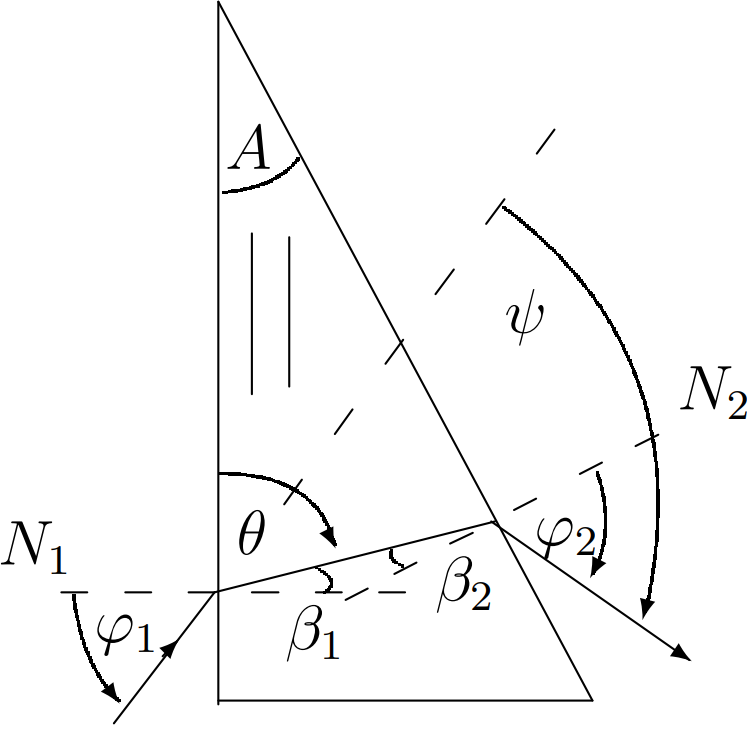
\includegraphics[width=\linewidth]{pic/prism}
                \caption{Рис. 3: Преломление луча в призме}
                \label{fig:fig3}
            \end{minipage}
            \setcounter{enumii}{6}

            \item используя специальное ПО для обработки значений углов,
            получим оценки для главных показателей преломления
            \[n_o = (1.647 \pm 0.003) \quad \chi^2_o \approx 56\]
            \[n_e = (1.467 \pm 0.005) \quad \chi^2_e \approx 2\]
            \item при этом для принятия гипотезы, значения хи-квадрата должны быть меньше 20,
            то есть по проведенному нами эксперименту невозможно принять гипотезу
            о независимости главного показателя преломления $n_o$ от угла $\theta$.
        \end{enumerate}
    \end{enumerate}

    \subsection*{Выводы}
    \begin{itemize}[label=\ding{70}]
        \item В данной работе приведена оценка преломляющего угла призмы из исландского шпата
        \[A = (38.8 \pm 0.2)\;^{\circ}.\]
        \item Был проведен эксперимент для оценки главных показателей преломления одноосного кристалла
        \[n_o = (1.647 \pm 0.003) \quad \chi^2_o \approx 56\]
        \[n_e = (1.467 \pm 0.005) \quad \chi^2_e \approx 2\]
        значения отличаются от табличных
        \[n_o_{\text{табл}} = 1.655\]
        \[n_e_{\text{табл}} = 1.485\]
        это может говорить о том, что погрешности в работе были занижены или наш образец отличается от эталона.
        \item Ожидания подкрепленные теоретическими выкладками подтвердились частично: гипотеза о том,
        что показатель преломления в случае обыкновенной волны не зависит от угла поворота призмы $\theta$
        не подтвердилась, тогда как гипотеза о зависимости показателя преломления в случае
        необыкновенной волны (см. уравнения\ \eqref{eq:eq6},\ \eqref{eq:eq7}) подтвердилась.
        \item Причем график (см. Приложение), построенный для случая обыкновенной волны,
        показывает зависимость похожую на зависимость в случае необыкновенной волны.
        Это может говорить о том, что падающий на призму луч лазера который,
        как считалось параллелен верхней поверхности кристала, был направлен под некоторым углом к горизонту.
        То есть несогласование эксперимента с теорией могло произойти из-за неточной юстировки.
    \end{itemize}

    \begin{table}[b]
        \centering
        \caption{Измерение преломляющего угла А призмы}
        \label{tab:tab1}
        \begin{tabular}{|p{0.5cm}|p{3cm}|p{4cm}|p{4cm}|}
            \hline
            {} & Лимб (отраженный луч), $^{\circ}$ & Риска (отражение от длинного катета), $^{\circ}$ & Риска (отражение от гипотенузы), $^{\circ}$ \\\hline
            0  & 10                                & 65                                               & 283                                         \\
            1  & 20                                & 70                                               & 289                                         \\
            2  & 30                                & 75                                               & 293                                         \\
            3  & 40                                & 80                                               & 299                                         \\
            4  & 50                                & 85                                               & 304                                         \\
            5  & 60                                & 90                                               & 308                                         \\
            6  & 70                                & 95                                               & 314                                         \\
            7  & 80                                & 100                                              & 319                                         \\
            8  & 90                                & 105                                              & 324                                         \\
            9  & 100                               & 110                                              & 329                                         \\
            10 & 110                               & 115                                              & 334                                         \\
            11 & 120                               & 120                                              & 339                                         \\
            12 & 130                               & 130                                              & 344                                         \\
            13 & 140                               & 140                                              & 349                                         \\\hline
        \end{tabular}
    \end{table}

    \begin{table}
        \centering
        \caption{Измерение главных показателей преломления $n_o,\ n_e$}
        \label{tab:tab2}
        \begin{tabular}{|p{0.5cm}|p{3cm}|p{4cm}|p{4cm}|}
            \hline
            {} & Отраженный луч & Преломленный обыкновенный луч & Преломленный необыкновенный луч \\\hline
            0  & 20             & 212.5                         & 203.0                           \\
            1  & 30             & 210.5                         & 202.0                           \\
            2  & 40             & 209.0                         & 201.8                           \\
            3  & 50             & 208.5                         & 201.5                           \\
            4  & 60             & 208.0                         & 202.0                           \\
            5  & 70             & 208.0                         & 202.5                           \\
            6  & 80             & 209.0                         & 203.0                           \\
            7  & 90             & 210.0                         & 204.5                           \\
            8  & 100            & 211.0                         & 206.0                           \\
            9  & 110            & 213.0                         & 208.0                           \\
            10 & 120            & 215.0                         & 210.0                           \\
            11 & 130            & 217.0                         & 212.5                           \\
            12 & 140            & 220.5                         & 215.5                           \\\hline
        \end{tabular}
    \end{table}
\end{document}